\documentclass{exam}

\usepackage{units} 
\usepackage[fleqn]{amsmath}
\usepackage{float}
\usepackage{mdwlist}
\usepackage{booktabs}
\usepackage{caption}
\usepackage{fullpage}
\usepackage{enumerate}
\usepackage{graphicx}

\usepackage{2in1, lscape} 

\everymath{\displaystyle}

\printanswers

\title{Statistics \\ Week Four}
\date{\today}
\author{}

\begin{document}

\maketitle
\tableofcontents

  \section{Homework}

  \begin{itemize*}
    \item do problem 30
    \item Sorry about problem 32. I didn't mean to assign such a tedious problem.  
    \item Try to be a little more in depth with descriptions and analysis.
  \end{itemize*}

  \section{Scatter Plots}

  \subsection{Notes}
  \begin{itemize*}
    \item show relationship between two quantitative variables
    \item each data point is an observation
    \item if one thing may be causing the other, put cause on x-axis and result on y-axis
    \item units can be different
    \item when variables are correlated, the points in a scatter plot tend to gather
      around the SD line.  The SD line 
      \begin{itemize*}
        \item goes through $(\bar{x}, \bar{y})$
        \item has slope $\pm \frac{s_y}{x_x}$
      \end{itemize*}
  \end{itemize*}

  \subsection{Correlation Doesn't Imply Causation}  

  The relationship may be coincidental.  For example, from 1980-1995 violent crime
  and CD sales both increased dramatically.  The relationship is probably
  coincidental.  

  To prove that smoking causes disease, you have to eliminate potential confounding
  factors like:
  \begin{itemize*}
    \item smokers tend to live in cities and are exposed to more pollution
    \item smokers are more often men, and men are more prone to heart disease
    \item long-time smokers tend to be older, and older people tend to get cancer
    \item is there some gene that both causes cancer and causes people to want to
      smoke?
  \end{itemize*}

  The relationship may be due to a ``confounding factor.''  For example, UBB has a
  strong negative correlation with recidivism, but some part of the explanation is
  that UBB attracts students who are unlikely recidivism candidates anyway.   The
  confounding factor is that UBB may just be identifying prisoners who are already
  low-recidivism risks, rather than reducing the recidivism risk for high-risk
  prisoners.

  \section{Correlation Coefficient}
  \[
    r = \frac{1}{n - 1} \sum z_x z_y
  \]

  \begin{itemize*}
    \item numerical measure of strength of relationship between two quantitative
      variables

    \item draw picture of quadrants, +/+ in Q1 and -/- in Q2

    \item sum of products of z-scores

    \item $-1 \leq r \leq 1$

    \item 1 means exact positive correlation, -1 means exact negative correlation

    \item if the correlation is high (absolute value), knowing the value of one
      variable allows you to fairly accurately guess the value of the other one

    \item correlation doesn't mean causation.  

    \item adding constant to every term just shifts line up, doesn't change
      correlation

  \end{itemize*}

  if x and y match exactly:
  \begin{align*}
    r & = \frac{1}{n - 1} \sum z_x z_x \\
      & = \frac{1}{n - 1} \sum \frac{x_i - \bar{x}}{s_x} \cdot \frac{x_i - \bar{x}}{s_x} \\
      & = \frac{1}{n - 1} \sum \frac{(x_i - \bar{x})^2}{s_x^2} \\
      & = \frac{1}{n - 1} \sum \frac{(n - 1) s_x^2}{s_x^2} \\
      & = \frac{n - 1}{n - 1} \\
      & = 1 \\
  \end{align*}

  \section{Examples}

  \begin{enumerate}
    \item find the correlation coefficient:
      \begin{table}[ht]
      \centering
      \begin{tabular}{rrrr}
        \toprule
        \multicolumn{2}{c}{Raw} & \multicolumn{2}{c}{z-score } \\
        \cmidrule(r){1-2} \cmidrule(r){3-4} 
        x & y & x     & y \\
        \midrule
        1 & 6 & -1.39 & 0.93 \\
        2 & 7 & -0.93 & 1.39 \\
        3 & 5 & -0.46 & 0.46 \\
        4 & 4 & 0.00  & 0.00 \\
        5 & 3 & 0.46  & -0.46 \\
        6 & 1 & 0.93  & -1.39 \\
        7 & 2 & 1.39  & -0.93 \\
        \bottomrule
      \end{tabular}
      \end{table}

    \begin{solution}
      \begin{align*}
        m &= 4 \\
        s &= 2.16 \\
        r &= -0.9286
      \end{align*}
    \end{solution}

    \item find the correlation coefficient:
      \begin{table}[ht]
      \centering
      \begin{tabular}{rrrr}
        \toprule
        \multicolumn{2}{c}{Raw} & \multicolumn{2}{c}{z-score } \\
        \cmidrule(r){1-2} \cmidrule(r){3-4} 
        x & y & x     & y \\
        \midrule
        1 & 2 & -1.39 & -0.93 \\ 
        2 & 1 & -0.93 & -1.39 \\ 
        3 & 4 & -0.46 & 0.00 \\ 
        4 & 3 & 0.00 & -0.46 \\ 
        5 & 7 & 0.46 & 1.39 \\ 
        6 & 5 & 0.93 & 0.46 \\ 
        7 & 6 & 1.39 & 0.93 \\ 
        \bottomrule
      \end{tabular}
      \end{table}

    \begin{solution}
      \begin{align*}
        m &= 4 \\
        s &= 2.16 \\
        r &= 0.8214 \\
      \end{align*}
    \end{solution}

    \item find the correlation coefficient:
      \begin{table}[ht]
      \centering
      \begin{tabular}{rrrr}
        \toprule
        \multicolumn{2}{c}{Raw} & \multicolumn{2}{c}{z-score } \\
        \cmidrule(r){1-2} \cmidrule(r){3-4} 
        x & y & x     & y \\
        \midrule
        1 & 7 & -1.39 & 1.39 \\ 
        2 & 6 & -0.93 & 0.93 \\ 
        3 & 5 & -0.46 & 0.46 \\ 
        4 & 4 & 0.00 & 0.00 \\ 
        5 & 3 & 0.46 & -0.46 \\ 
        6 & 2 & 0.93 & -0.93 \\ 
        7 & 1 & 1.39 & -1.39 \\ 
        \bottomrule
      \end{tabular}
      \end{table}

    \begin{solution}
      \begin{align*}
        m &= 4 \\
        s &= 2.16 \\
        r &= -1 \\
      \end{align*}
    \end{solution}

    \item If men always married women 8 inches shorter, what would the correlation
      between their heights be?
      
      \begin{solution}
        1, because it just changes the scale on the y-axis
      \end{solution}

    \item If men always married women 8\% shorter, what would the correlation
      between their heights be?
      \begin{solution}
        1, because it just changes the scale on the y-axis
      \end{solution}

    \item Match correlations with data:
      data:
      \begin{itemize*}
        \item GPA for freshman year and sophomore year
        \item GPA for freshman year and senior year
        \item length and weight of 2x4s
      \end{itemize*}

      \begin{itemize*}
        \item 0.95
        \item 0.60
        \item 0.30
      \end{itemize*}

  \end{enumerate}

  \section{NFL}

  \subsection{Passing Attempts vs. Yards}

  \begin{table}[H]
    \centering
      \begin{tabular}{rrrrr}
        \toprule
           & \multicolumn{2}{c}{Raw} & \multicolumn{2}{c}{z-score } \\
        \cmidrule(r){2-3} \cmidrule(r){4-5} 
           & Attempts & Yards & Attempts & Yards \\
        \midrule
        1  & 17       & 70    & -1.80    & -1.86 \\
        2  & 40       & 305   & 1.16     & 1.53 \\
        3  & 34       & 248   & 0.39     & 0.71 \\
        4  & 33       & 175   & 0.26     & -0.35 \\
        5  & 40       & 266   & 1.16     & 0.96 \\
        6  & 26       & 124   & -0.64    & -1.08 \\
        7  & 24       & 138   & -0.90    & -0.88 \\
        8  & 39       & 277   & 1.03     & 1.12 \\
        9  & 21       & 144   & -1.28    & -0.79 \\
        10 & 43       & 212   & 1.54     & 0.19 \\
        11 & 33       & 209   & 0.26     & 0.14 \\
        12 & 25       & 189   & -0.77    & -0.15 \\
        13 & 33       & 286   & 0.26     & 1.25 \\
        14 & 24       & 126   & -0.90    & -1.05 \\
        15 & 33       & 217   & 0.26     & 0.26 \\
        \bottomrule
      \end{tabular}
  \end{table}

  \begin{table}[ht]
    \centering
    \begin{tabular}{rlrr}
      \toprule
        & variable & mean   & sd \\
      \midrule
      1 & pa       & 31.00  & 8.00 \\
      2 & py       & 199.00 & 69.00 \\
      \bottomrule
    \end{tabular}
  \end{table}

  correlation coefficient: $r = 0.8450$

  \begin{figure}[H]
    \centering
    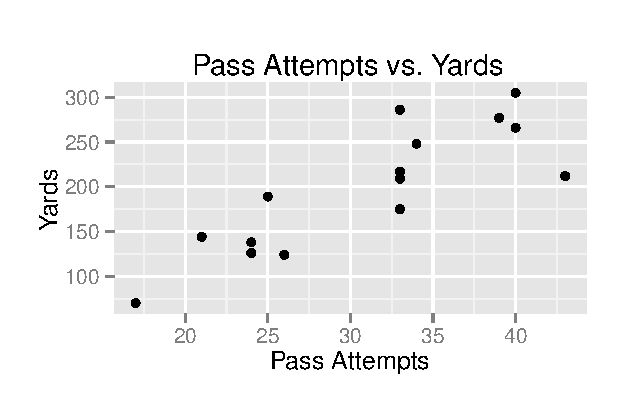
\includegraphics{figures/nfl/passing_attempts_vs_yds.eps}
    \caption{Passing attempts vs. yards}
  \end{figure}

  \subsection{Passing vs. Rushing}

  \begin{figure}[H]
    \centering
    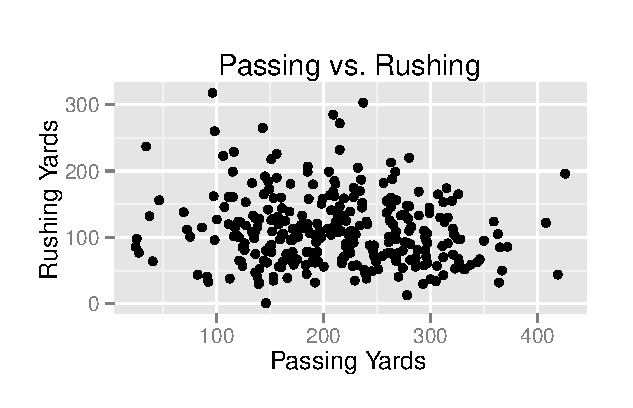
\includegraphics{figures/nfl/passing_vs_rushing.eps}
    \caption{Passing vs. Rushing}
  \end{figure}

  correlation coefficient: $r = -0.1342$

  \subsection{Punts vs. Points}

  \begin{figure}[H]
    \centering
    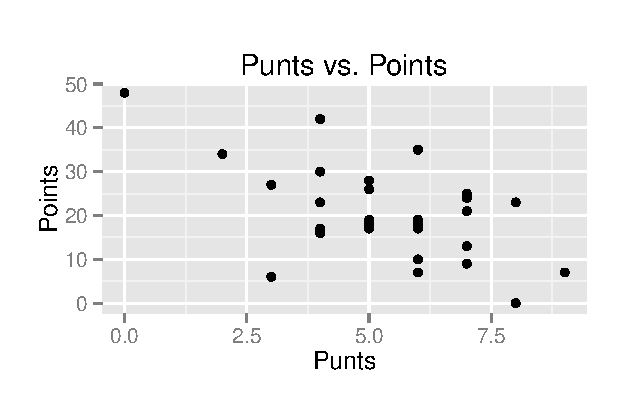
\includegraphics{figures/nfl/punts_vs_points.eps}
    \caption{Punts vs. Points}
  \end{figure}

  \begin{itemize*}
    \item correlation coefficient (sample): $r = -0.5751$
    \item correlation coefficient (all games): $r = -0.3793$
  \end{itemize*}

  \subsection{Turnover Differential}

  \begin{table}[H]
    \centering
    \begin{tabular}{rrrrr}
      \toprule
         & \multicolumn{2}{c}{Raw} & \multicolumn{2}{c}{z-score } \\
      \cmidrule(r){2-3} \cmidrule(r){4-5} 
         & Turnovers & Points & Turnovers & Points \\
      \midrule
      1  & 1         & -8     & 0.64      & -0.43 \\
      2  & -1        & -5     & -0.37     & -0.23 \\
      3  & 0         & -2     & 0.14      & -0.03 \\
      4  & 1         & 21     & 0.64      & 1.48 \\
      5  & 1         & 7      & 0.64      & 0.56 \\
      6  & 1         & 3      & 0.64      & 0.30 \\
      7  & 0         & -12    & 0.14      & -0.69 \\
      8  & -1        & -18    & -0.37     & -1.08 \\
      9  & 3         & 10     & 1.66      & 0.76 \\
      10 & -1        & -4     & -0.37     & -0.16 \\
      11 & 0         & 10     & 0.14      & 0.76 \\
      12 & -2        & -17    & -0.88     & -1.02 \\
      13 & 1         & 34     & 0.64      & 2.33 \\
      14 & 1         & 5      & 0.64      & 0.43 \\
      15 & -4        & -16    & -1.90     & -0.95 \\
      16 & 3         & 19     & 1.66      & 1.35 \\
      17 & -1        & -23    & -0.37     & -1.41 \\
      18 & 1         & -9     & 0.64      & -0.49 \\
      19 & -3        & -3     & -1.39     & -0.10 \\
      20 & 1         & -11    & 0.64      & -0.62 \\
      21 & -5        & -20    & -2.41     & -1.21 \\
      22 & 2         & 16     & 1.15      & 1.15 \\
      23 & 0         & 3      & 0.14      & 0.30 \\
      24 & -1        & -7     & -0.37     & -0.36 \\
      25 & -2        & -16    & -0.88     & -0.95 \\
      26 & -2        & -10    & -0.88     & -0.56 \\
      27 & -2        & 3      & -0.88     & 0.30 \\
      28 & -2        & -22    & -0.88     & -1.35 \\
      29 & 3         & 33     & 1.66      & 2.27 \\
      30 & 0         & -6     & 0.14      & -0.30 \\
       \bottomrule
    \end{tabular}
  \end{table}

  \begin{figure}[H]
    \centering
    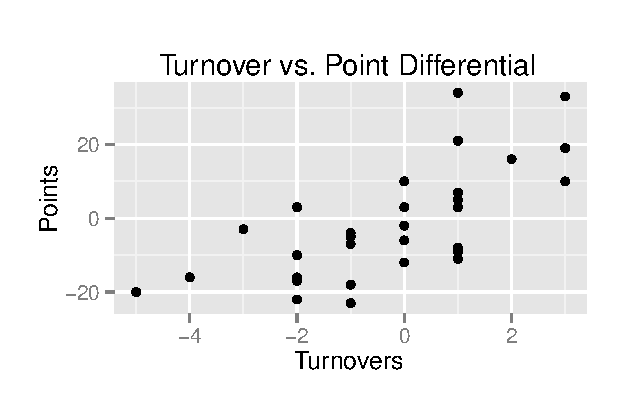
\includegraphics{figures/nfl/to_vs_pts.eps}
    \caption{Turnovers vs. Points (sample)}
  \end{figure}

  \begin{table}[H]
    \centering
    \begin{tabular}{rlrr}
      \toprule
         & variable & mean & s \\
      \midrule
      1  & to       & 0.03 & 1.54 \\
      2  & pts      & 1.17 & 14.88 \\
      \bottomrule
    \end{tabular}
    \caption{Statistics for sample}
  \end{table}

  \begin{itemize*}
    \item correlation coefficient: $r = 0.6941$
    \item correlation coefficient (all games): $r = 0.5683$
  \end{itemize*}

  \begin{figure}[H]
    \centering
    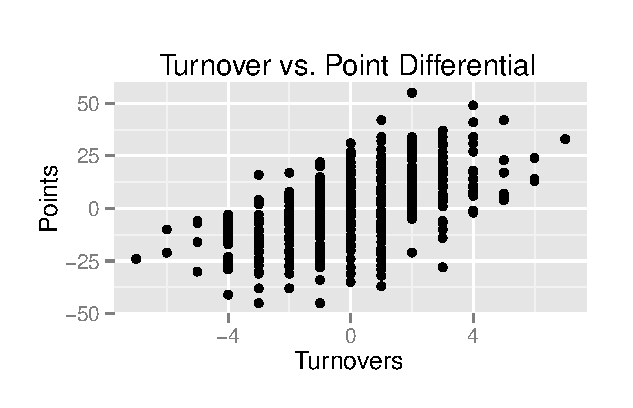
\includegraphics{figures/nfl/to_vs_pts_all.eps}
    \caption{Turnovers vs. Points (large sample)}
  \end{figure}

  \section{Crime and Incarceration Rates}

  \begin{figure}[H]
    \centering
    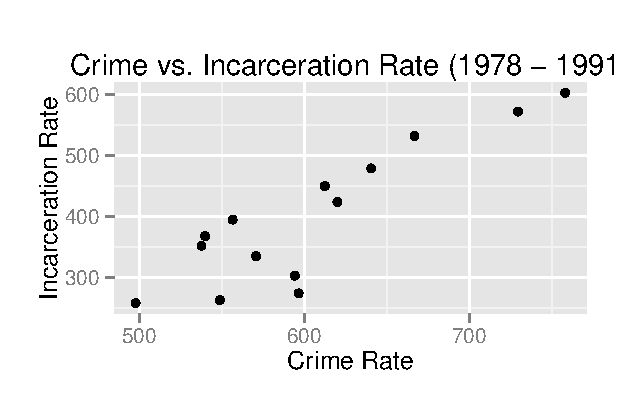
\includegraphics{figures/crime/crime_vs_incarceration_1978-1991.eps}
    \caption{1978 - 1991}
  \end{figure}

  \begin{figure}[H]
    \centering
    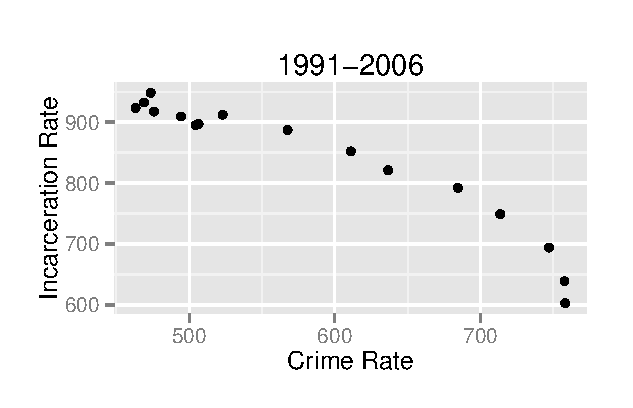
\includegraphics{figures/crime/crime_vs_incarceration_1991-2006.eps}
    \caption{1991 - 2006}
  \end{figure}

  \begin{figure}[H]
    \centering
    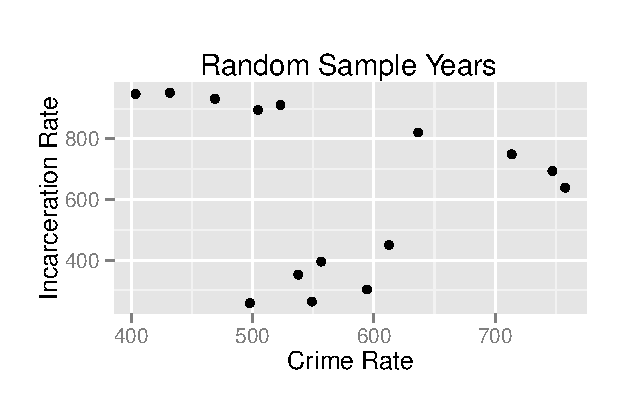
\includegraphics{figures/crime/crime_vs_incarceration_sample.eps}
    \caption{Random Years}
  \end{figure}

\end{document}

